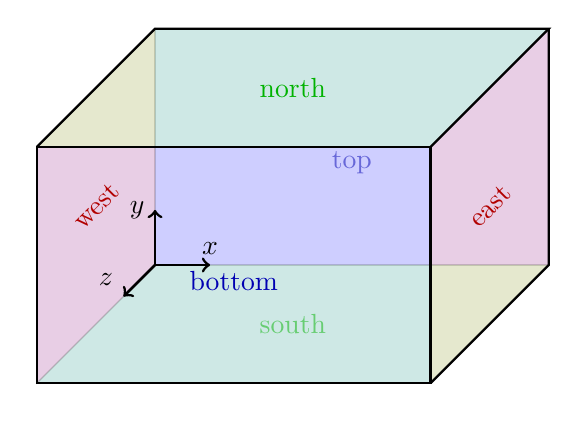
\begin{tikzpicture}
        \node (-0.1, -0.1) {};
        \draw[fill=blue, opacity=0.1] (0,0) -- (0,3) -- (5,3) -- (5,0) -- cycle;
        \draw[fill=blue, opacity=0.1] (1.5,1.5) -- (1.5,4.5) -- (6.5,4.5) -- (6.5,1.5) -- cycle;
        \draw[fill=red, opacity=0.1] (5,0) -- (5,3) -- (6.5,4.5) -- (6.5,1.5) -- cycle;
        \draw[fill=red, opacity=0.1] (0,0) -- (0.0,3.0) -- (1.5,4.5) -- (1.5,1.5) -- cycle;
        \draw[fill=green, opacity=0.1] (0,0) -- (1.5,1.5) -- (6.5,1.5) -- (5,0) -- cycle;
        \draw[fill=green, opacity=0.1] (0,3) -- (1.5,4.5) -- (6.5,4.5) -- (5,3) -- cycle;
        \draw[thick] (0,0) -- (0,3) -- (5,3) -- (5,0) -- cycle;
        \draw[thick] (0,3) -- (1.5,4.5) -- (6.5,4.5) -- (5,3);
        \draw[thick] (5,0) -- (6.5,1.5) -- (6.5,4.5);
        \node[opacity=0.5] at (3.25,0.75) {\textcolor{green!70!black}{south}};

        \node[opacity=0.5] at (4,2.8) {\textcolor{blue!70!black}{top}};
        \draw[draw=none] (0.0,1.5) -- (1.5,3.0) node[midway, sloped] {\textcolor{red!70!black}{west}};
        \draw[draw=none] (5.0,1.5) -- (6.5,3.0) node[midway, sloped] {\textcolor{red!70!black}{east}};
        \draw[line width=1pt, ->] (1.5,1.5) -- (2.2,1.5) node[at end, above] {$x$};
        \draw[line width=1pt, ->] (1.5,1.5) -- (1.5,2.2) node[at end, left] {$y$};
        \draw[line width=1pt, ->] (1.5,1.5) -- (1.1,1.1) node[at end, above left] {$z$};
        \node at (3.25,3.75) {\textcolor{green!70!black}{north}};
        \node at (2.5,1.3) {\textcolor{blue!70!black}{bottom}};
    \end{tikzpicture}